\documentclass[a4paper,12pt]{article}
\usepackage[latin1]{inputenc}
\usepackage[spanish]{babel}
\usepackage{bm}
\usepackage{graphicx}
\usepackage{amsmath}
\setlength{\textheight}{235mm}
\setlength{\textwidth}{168mm}
\setlength{\oddsidemargin}{0pt}
\pagestyle{empty}
\begin{document}
\mbox{}\vspace*{-45mm}

{\centering
{\small\sc Escuela T�cnica Superior de Ingenieros de Caminos, Canales y
Puertos (Madrid)}\\*[4mm]
{\Large\bf M�todo de los Elementos Finitos (Curso 22-23)}\\*[4mm]
Ejercicio 4: Tecnolog�a de Elementos\\*[4mm]

}

\vspace{3mm}

%%%%%
La estructura del puente mostrada en la figura inferior se encuentra sujeta a una presi�n vertical de $1$ MPa en su parte superior por efecto de cargas externas. El material tiene un m�dulo de elasticidad $E=22$ GPa, coeficiente de Poisson $\nu=0.30$, y un peso espec�fico de $\gamma=25000$ N/m$^3$.  La base de los pilares se asume como empotrada y los lados laterales tienen simetr�a en la direcci�n del eje del puente. La estructura tiene un espesor de $0.50$ m. Considerando el modelado de la mitad derecha de uno de los pilares (tener en cuenta las condiciones de simetr�a) y el efecto de todas las cargas (de gravedad y externas), se pide resolver la estructura con un mallado de $0.25$ m de tama�o y tipo de elemento C3D8.
\\

\begin{center}
	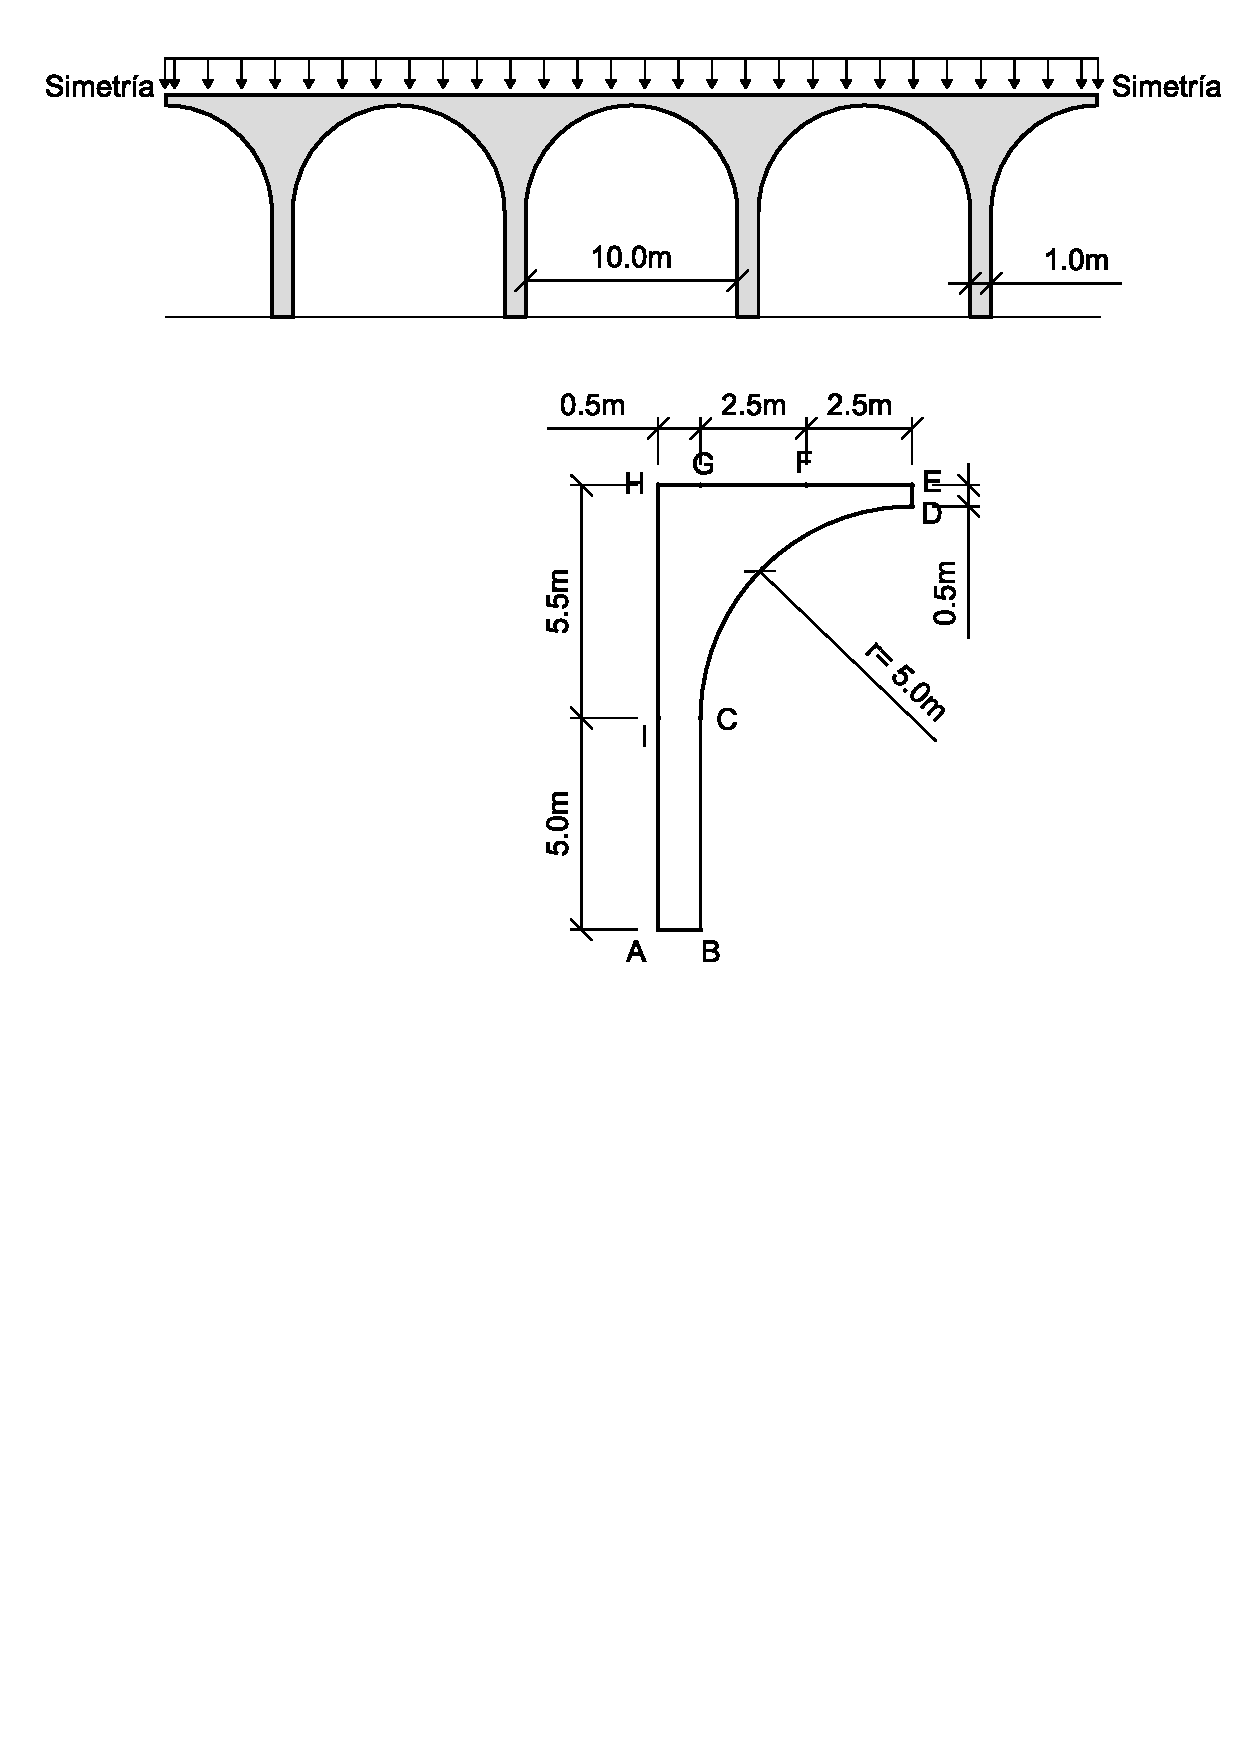
\includegraphics[width=0.82\textwidth]{figura}
\end{center}
\end{document}
